
\documentclass[
11pt,
titlepage,
a4paper,
ngerman,
captions=tableheading,
toc=bibliography,
%toc=listof,
numbers=noenddot
] {scrartcl}

\usepackage{ifpdf}
\usepackage[T1]{fontenc}
\usepackage[utf8]{inputenc}
\usepackage{microtype}
\usepackage{amsmath, amssymb, amstext}
%\usepackage{palatino}            % andere Schriftart
\usepackage[ngerman]{babel}       % Deutsch !
\usepackage[babel, german=quotes]{csquotes}
\usepackage{color}
\usepackage{graphicx}             % Bilder einbinden ermöglichen
\usepackage[obeyspaces]{url}                  % Besserew
\usepackage[textsize=small, textwidth=0.8in]{todonotes} % \todo noch zu tun
\usepackage{multirow}             % Zusammenfassen von Tabellenzellen
\usepackage{upgreek}              % nicht-kursive Griechische Buchstaben
\usepackage{textcomp}             % \textperthousand  (promille)
\usepackage{rotating}             % rotierte Information
\usepackage[format=plain, indention=1cm, scriptsize,font=sf, labelfont=bf, nooneline]{caption}
\usepackage{subfigure}%veraltet??
                                  % modif Bildunterschriften
\renewcommand{\captionfont}{\small \sffamily \slshape}
\renewcommand{\captionlabelfont}{\small \sffamily \slshape \bfseries   }

\usepackage[section]{placeins}
\usepackage{pdflscape}

%Einheiten
\usepackage[separate-uncertainty = true, locale=DE, alsoload=synchem]{siunitx}
\DeclareSIUnit{\ev}{\text{eV}}
\DeclareSIUnit{\u}{\text{u}}
\usepackage{units}

% Kontrolle der Seitenränder:
\usepackage[inner=3.5cm, outer=3cm, top=3cm, bottom=2cm, includehead, includefoot]{geometry}
% Besser nicht global als Standard setzen
%\clubpenalty=10000   % letzte Zeile einer Seite nicht erste Zeile eines Absatzes
%\widowpenalty=10000  % letzte Zeile eines Absatzes nicht erste Zeile einer Seite

% Eigene Kopf/Fußzeilen
\usepackage{fancyhdr}
\pagestyle{fancy}

% Standard:
\fancyhead[EL]{\thepage}
\fancyhead[ER]{\slshape \nouppercase{\leftmark}}
\fancyhead[OL]{\slshape \nouppercase{\leftmark}}
\fancyhead[OR]{\thepage}

% Fußzeile: Datum,  Seine X von Y, gut während des Schreibens:
\fancyfoot[EC, OC]{}%{\today{} $\ \ast\ast\ast\ $ Seite \thepage{}  von \pageref{LastPage}}

%neue Pakete
\usepackage{ae}
\usepackage{icomma}

\usepackage{hyperref}                            %macht anklickbare Links
\definecolor{LinkColor}{rgb}{0,0,0.75}           %dunkelblau
%\definecolor{LinkColor}{rgb}{0,0,0}             %schwarz

\hypersetup{
	pdftitle = {LaTeX-Vorlage},
	pdfsubject = {LaTeX-Vorlage},
	pdfkeywords = {LaTeX, Vorlage, Uni Wuppertal},
	pdfauthor = {Ich},
	bookmarksnumbered = true,
	bookmarksopen = false,
	colorlinks = false,
	hypertexnames = true,
	a4paper = true,
	colorlinks=true,%
	linkcolor=LinkColor,%
	citecolor=LinkColor,%
	filecolor=LinkColor,%
	menucolor=LinkColor,%
	urlcolor=LinkColor,
	breaklinks=true
}

%%%%Codedarstellung
% Custom colors
\usepackage{color}
\definecolor{deepblue}{rgb}{0,0,0.5}
\definecolor{deepred}{rgb}{0.6,0,0}
\definecolor{deepgreen}{rgb}{0,0.5,0}
\definecolor{bgcolor}{rgb}{0.95,0.95,0.95}

\usepackage{listings}

% Python style for highlighting
\newcommand\codestyle[1]{\lstset{
language=#1,
%basicstyle=\ttm,
otherkeywords={self},             % Add keywords here
%keywordstyle=\ttb\color{deepblue},
emph={MyClass,__init__,rld},          % Custom highlighting
emphstyle=\ttfamily\color{deepblue},    % Custom highlighting style
%stringstyle=\color{deepgreen},
%frame=tb,                         % Any extra options here
showstringspaces=false,            %
%%
keywordstyle=\bfseries\ttfamily\color{deepred},
identifierstyle=\ttfamily\color{black},
commentstyle=\color[RGB]{120, 191, 142},
stringstyle=\ttfamily\color[rgb]{0.81,0.17,0},%[RGB]{deepgreen},%[rgb]{0.627,0.126,0.941},{164,196,0}
basicstyle= \ttfamily\footnotesize\color[RGB]{49,102,145},
numberstyle=\scriptsize\color{black},
numbers=left,
stepnumber=1,
numbersep=10pt,
tabsize=2,
breaklines=true,
%prebreak = \raisebox{0ex}[0ex][0ex]{\ensuremath{\hookleftarrow}},
breakatwhitespace=false,
aboveskip={1.5\baselineskip},
  columns=fixed,
  upquote=true,
  extendedchars=true,
 frame=single,
rulecolor=\color{black},
backgroundcolor=\color{bgcolor},
}}


% External codefiles
\newcommand\codefile[3][,]{{
\codestyle{#2}
\lstinputlisting[#1]{#3}
}}

%%%%%

%%neue Kommandos
\newenvironment{changemargin}[2]{%
\begin{list}{}{%
\setlength{\topsep}{0pt}%
\setlength{\leftmargin}{#1}%
\setlength{\rightmargin}{#2}%
\setlength{\listparindent}{\parindent}%
\setlength{\itemindent}{\parindent}%
\setlength{\parsep}{\parskip}%
}%
\item[]}{\end{list}}

%Sachen nebeneinander packen + \parindent Fox
\newlength{\myParindent} %Zwischenspeicher für \parindent
\setlength{\myParindent}{\the\parindent}

\newcommand{\colw}{0.63\linewidth}% ändern mit \renewcommand
\newcommand{\colmarg}{-1.2cm}
\newcommand{\twocol}[2]{
\begin{changemargin}{\colmarg}{\colmarg + 0.5cm}
\begin{minipage}{\colw}
#1
\end{minipage}
\begin{minipage}{\linewidth - \colw}
#2
\end{minipage}
\end{changemargin}
}
\newcommand{\colcap}[1]{ %setzt irgendwie \parindent auf 0, kA was das noch alles verhaut.
\vspace{-1.6em}
\captionof{figure}{#1}
\vspace{1.4em}
\setlength{\parindent}{\the\myParindent} %daher alten Wert zurücksetzen
}
\newcommand{\resetcol}{
\renewcommand{\colmarg}{-1.2cm}
\renewcommand{\colw}{0.63\linewidth}
}

\newcommand{\ufrac}[3]{\SI{#1}{$\unit{\frac{#2}{#3}}$} }
\newcommand{\PM}{&\hspace{-0,3cm}$\pm$&\hspace{-0,3cm}}


\newcommand{\gq}[1]{\glqq #1\grqq ~} %German Quotes

%%%%%%%%%%%%%%%%%%%%%%%%%%%%%%%%%%%%%%%%%%%%%%%%%%%%%%%%%%%%%%%
\newcommand{\ttt}[1]{\verb|#1|} %Code Schrift
\DeclareUrlCommand\ttt{\texttt{\urlstyle{same}}}

% \newcommand{\codesize}[1]{ basicstyle= {\ttfamily#1\color[RGB]{49,102,145}} }
%\newcommand{\codesize}[1]{ \ttfamily#1\color[RGB]{49,102,145} }
\newcommand{\codesize}[1]{ \lstset{ basicstyle= {\ttfamily#1\color[RGB]{49,102,145}} } }

%\newenvironment{nrcode}{\lstlisting}}{\endlstlisting}
%\renewcommand\lstlistingname{Programm} %umbenennen??
%[numbers=left, frame=single]
\lstnewenvironment{nrcode}[1][,]{
\lstset{numbers=left, frame=single, #1}
}{}

\newenvironment{source}{\quote}{\endquote}

%%Inline-Code-Setup
\newcommand{\inlinecodestyle}[1]{
\codestyle{#1}
\lstset{numbers=none , frame=none, basicstyle= \ttfamily\small\color[RGB]{49,102,145}, aboveskip={0.5\baselineskip}}%, backgroundcolor=\color{white}}
}

\lstset{escapeinside={\#(*}{*)}} %fuer labels!
%%%%%%%%%%%%%%%%%%%%%%%%%%%%%%%%%%%%%%%%%%%%%%%%%%%%%%%%%%%%%%%

% Stil der Zitate und der Bibliographie
\usepackage[style=numeric, backend=biber, bibencoding=utf8, bibwarn=true, sorting=none
			%, hyperref=true, backref=true
]{biblatex}
\addbibresource{literatur.bib}



\title{ Einfacher? Crosscompiler von Python nach C++ }
\subject{Programmierpraktikum}
\author{Felix Helsch \\ Julian Buchhorn}
\date{\today}

\publishers{\parbox[b][8cm]{\textwidth}{\centering \textbf{Betreuer}\\Dr. Holger Arndt}}

\usepackage[version=3]{mhchem}
\usepackage{rotating}
\usepackage{booktabs}

\newcommand{\cc}[1]{\multicolumn{1}{c}{#1}} %Cell-Center
\newcommand{\C}[2]{\multicolumn{#1}{|c|}{#2}} %multiCol-wall
\newcommand{\mc}[2]{\multicolumn{#1}{c}{#2}} %multicol

\inlinecodestyle{python}
\lstset{ escapeinside= {\#(*} {*)} }
\lstset{
 rangeprefix= \#\\*,
 includerangemarker= false,
 texcl= false, %??
}
%%%%%%%%%%%%%%%%%%%%%%%%%%%%%%%%%%%%%%%%%%%%%%%%%%%%%%%%%%%%%%%%%%%%%%
\begin{document}                                       

\pagestyle{empty}
\maketitle
\tableofcontents

\clearpage 
\pagestyle{fancy}
%%%%%%%%%%%%%%%%%%%%%%%%%%%%%%%%%%%%%%%%%%%%%%%%%%%%%%%%%%%%%%%%%%%%%%

\section{Einleitung}

Im Rahmen eines Programmierpraktikums an der bergischen Universität Wuppertal haben wir einen Compiler von Python zu C++ geschrieben. Dabei ging es in erster Linie darum, zu verstehen, wie ein Compiler funktioniert und nicht einen vollständigen Compiler zu schreiben.

Als vorläufiges Ziel hatten wir uns gesetzt ein einfaches Testprogramm mit grundlegenden Syntaxelementen zu übersetzen (s. Lst. \ref{pyprog}).

\codefile[caption= Python Testprogramm für den Compiler, label=pyprog]{python}{program.py}

Das Ziel haben wir erreicht, unser Compiler kann in seinem momentanen Zustand das Python Programm übersetzen und liefert das C++ Programm in Listing \ref{cppprog}. Dabei mussten wie erwartet einige Annahmen über das Programm gemacht werden um die Übersetzung zu vereinfachen.

\codefile[caption= Vom Compiler erzeugtes C++ Programm, label=cppprog]{c++}{program.cpp}


In den folgenden Kapiteln werden wir noch erklären wie man den Compiler verwenden kann, welche Programme man dafür benötigt und welche Features der Compiler im Moment unterstützt. Zum Schluss werden wir noch kurz auf die Struktur des Codes eingehen, den wir geschrieben haben.

Für eine detailliertere Erklärung verweisen wir auf die Bachelorarbeit von Felix Helsch verwiesen..., in welcher die Erstellung des Compilers fortgeführt wird.

%%%%%%%%%%%%%%%%%%%%%%%%%%%%%%%%%%%%%%%%%%%%%%%%%%%%%%%%%%%%%%%%%%%%%%

\section{Verwendung}


%%%%%%%%%%%%%%%%%%%%%%%%%%%%%%%%%%%%%%%%%%%%%%%%%%%%%%%%%%%%%%%%%%%%%%

\section{Programme}


\begin{center}
 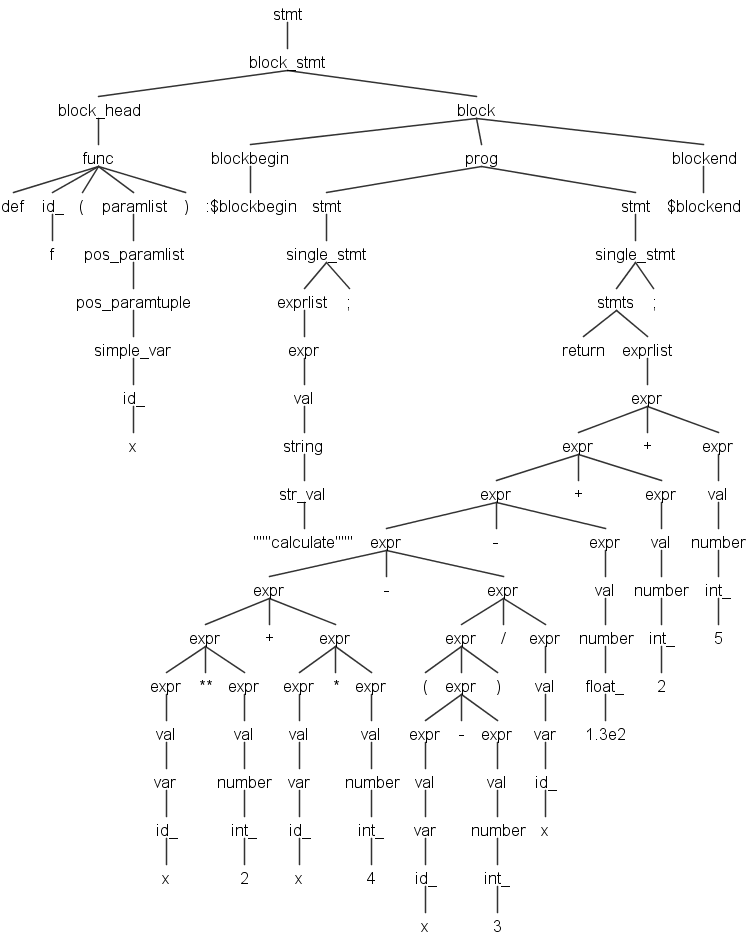
\includegraphics[width=0.8\linewidth]{Bilder/program_func_parse_tree2.png}
 \captionof{figure}{ Beispiel Parsetree }
\end{center}

%%%%%%%%%%%%%%%%%%%%%%%%%%%%%%%%%%%%%%%%%%%%%%%%%%%%%%%%%%%%%%%%%%%%%%

\section{Features}


%%%%%%%%%%%%%%%%%%%%%%%%%%%%%%%%%%%%%%%%%%%%%%%%%%%%%%%%%%%%%%%%%%%%%%

\section{Codestruktur}






%%%%%%%%%%%%%%%%%%%%%%%%%%%%%%%%%%%%%%%%%%%%%%%%%%%%%%%%%%%%%%%%%%%%%%
\appendix
\newpage
%%%%%%%%%%%%%%%%%%%%%%%%%%%%%%%%%%%%%%%%%%%%%%%%%%%%%%%%%%%%

\section{Programm... } \label{py}

%\codefile{python}{test.py}{caption=cap}

\codefile[caption=cap, label=pycode, linerange=s-e]{python}{test.py}







\clearpage
\listoffigures
\clearpage
\listoftables
\clearpage
\lstlistoflistings
\clearpage
\nocite{*}
\printbibliography

\end{document}
%%%%%%%%%%%%%%%%%%%%%%%%%%%%%%%%%%%%%%%%%%%%%%%%%%%%%%%%%%%%%%%%%%%%%%%%

\subsubsection*{Code Schrift}
Text mit \ttt{Code} \ttt{Schrift} .

\subsubsection*{Inline Code}
\begin{lstlisting}[caption=CAP]
inline code test
\end{lstlisting}

\vspace{4ex}
\subsubsection*{Numerierter Inline Code}
\begin{nrcode}[caption=CCC, label=pynr, linerange={a-c, d-e}]
import math
#\*a
2
nr code test #(*\label{txtline}*)
4
5
#\*b
6
7
#\*c
8
9
#\*d
10
11
#\*e
12
\end{nrcode}

Referenz für Code \ref{pynr} Zeile \ref{txtline}.

Referenz für Code \ref{pycode} Zeile \ref{test_arith}.